\documentclass{article}
\usepackage[a4paper,left=3cm, right=3cm, top=2cm, bottom=2cm]{geometry}
\usepackage{amsmath}
\usepackage{graphicx}
\usepackage{caption}
\usepackage{setspace}
\usepackage{xcolor}
\usepackage{titlesec}
\usepackage{amssymb}
\usepackage{tcolorbox}
\usepackage{wrapfig}

\graphicspath{{graph/}}
\title{11.3 The Integral Test and Estimates of Sums}
\date{}
\author{}
\setstretch{1.3} 

% \subsection* 형식 지정 (번호 없음)
\titleformat{name=\section, numberless}
  {\normalfont\large\bfseries\color{blue}}
  {}
  {0pt}
  {}
\geometry{a4paper, margin=1in}

\begin{document}
\maketitle

\begin{figure}[htbp]
    \centering
    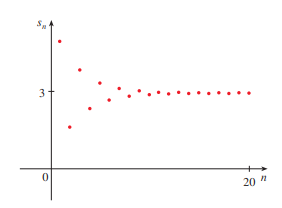
\includegraphics[width=0.35\textwidth]{graph72.png}
\end{figure} 

In general, it is difficult to find the exact sum of a series. In this section, we develop a test that enables us to determine whether a series is convergent or divergent without explicitly finding its sum.

\section*{The Integral Test}

\begin{tcolorbox}[
    colback=white,
    colframe=orange!80!white,
    title=The Integral Test,
    boxrule=0.5mm,
    arc=3mm
    ]
    Suppose \(f\) is a continuous, positive, decreasing function on \([1, \infty]\) and let \(a_n = f(n)\). Then the series \( \sum_{n=1}^{\infty} a_n \) is convergent if and only if the improper integral \( \int_1^\infty f(x) \,dx \) is convergent. In other words:
    \begin{itemize}
        \item[(i)] If \( \int_1^\infty f(x) \,dx \) is \textbf{convergent}, then \( \sum_{n=1}^{\infty} a_n \) is \textbf{convergent}.
        \item[(ii)] If \( \int_1^\infty f(x) \,dx \) is \textbf{divergent}, then \( \sum_{n=1}^{\infty} a_n \) is \textbf{divergent}.
    \end{itemize}
    \textbf{Note:} It is not necessary that \(f\) be always decreasing. It is sufficient if \(f\) is ultimately decreasing, i.e., decreasing for \(x\) larger than some number \(N\).
\end{tcolorbox}

\subsection*{EXAMPLE 1}
Test the series \( \sum_{n=1}^{\infty} \dfrac{1}{n^2+1} \) for convergence or divergence.\\
\textbf{SOLUTION:}
The function \(f(x) = \dfrac{1}{x^2+1}\) is continuous, positive, and decreasing on \([1, \infty]\) because \(x^2+1\) is an increasing function. We evaluate the integral:
\begin{align*}
    \int_1^\infty \dfrac{1}{x^2+1} \,dx &= \lim_{t\to\infty} \int_1^t \dfrac{1}{x^2+1} \,dx \\
    &= \lim_{t\to\infty} \left[ \tan^{-1}(x) \right]_1^t \\
    &= \lim_{t\to\infty} (\tan^{-1}(t) - \tan^{-1}(1)) = \dfrac{\pi}{2} - \dfrac{\pi}{4} = \dfrac{\pi}{4}
\end{align*}
Since this improper integral is convergent, the series is \textbf{convergent} by the Integral Test.

\section*{The p-series}
The series \( \sum_{n=1}^{\infty} \dfrac{1}{n^p} \) is called the \textbf{p-series}.

\begin{tcolorbox}[
    colback=white,
    colframe=orange!80!white,
    title=Convergence of a p-series,
    boxrule=0.5mm,
    arc=3mm
    ]
    The p-series \( \sum_{n=1}^{\infty} \dfrac{1}{n^p} \) is \textbf{convergent} if \(p > 1\) and \textbf{divergent} if \(p \le 1\).
\end{tcolorbox}

If \(p < 0\), then \( \lim_{n\to\infty} \dfrac{1}{n^p} = \lim_{n\to\infty} n^{-p} = \infty \) since \(-p > 0\).\\
If \(p = 0\), then \( \lim_{n\to\infty} \dfrac{1}{n^0} = \lim_{n\to\infty} 1 = 1 \). In either case, \( \lim_{n\to\infty} a_n \neq 0 \), so the given series diverges by the Test for Divergence.\\
If \(p > 0\), then the function \( f(x) = \dfrac{1}{x^p} \) is continuous, positive, and decreasing on \([1, \infty]\). We found in Section 7.8 that
$ \int_1^\infty \dfrac{1}{x^p} \,dx \quad \text{converges if } p > 1 \text{ and diverges if } p \le 1.$\\
It follows from the Integral Test that the series \( \sum 1/n^p \) converges if \(p > 1\) and diverges if \(0 < p \le 1\). (For \(p=1\), this series is the harmonic series, which we have already seen is divergent).


\subsection*{EXAMPLE 3}
(a) The series \( \sum_{n=1}^{\infty} \dfrac{1}{n^3} \) is convergent because it is a p-series with \(p = 3 > 1\). \\
(b) The series \( \sum_{n=1}^{\infty} \dfrac{1}{n^{1/3}} \) is divergent because it is a p-series with \(p = 1/3 < 1\).\\

\subsection*{EXAMPLE 4}
Determine whether the series \( \sum_{n=1}^{\infty} \dfrac{\ln n}{n} \) converges or diverges.\\
\textbf{SOLUTION:}
The function \(f(x) = \dfrac{\ln x}{x}\) is positive and continuous for \(x>1\). To check if it's decreasing, we find the derivative:
\[ f'(x) = \dfrac{x(1/x) - (\ln x)(1)}{x^2} = \dfrac{1 - \ln x}{x^2} \]
\(f'(x) < 0\) when \(1 - \ln x < 0\), or \(\ln x > 1\), which means \(x > e\). Thus, \(f\) is decreasing for \(x > e\).

Applying the Integral Test:
\[ \int_1^\infty \dfrac{\ln x}{x} \,dx = \lim_{t\to\infty} \left[ \dfrac{(\ln x)^2}{2} \right]_1^t = \lim_{t\to\infty} \dfrac{(\ln t)^2}{2} = \infty \]
The integral is divergent, so the series is \textbf{divergent}.

\section*{Estimating the Sum of a Series}
For a convergent series \( \sum a_n \), we can approximate its sum \(s\) with a partial sum \(s_n\). The error in this approximation is the remainder, \(R_n = s - s_n\).

\begin{tcolorbox}[
    colback=white,
    colframe=orange!80!white,
    title=Remainder Estimate for the Integral Test,
    boxrule=0.5mm,
    arc=3mm
    ]
    Suppose \(f(k) = a_k\), where \(f\) is a continuous, positive, decreasing function for \(x \ge n\) and \( \sum a_n \) is convergent. If \(R_n = s - s_n\), then:
    \[ \int_{n+1}^\infty f(x) \,dx \le R_n \le \int_n^\infty f(x) \,dx \]
\end{tcolorbox}

\subsection*{EXAMPLE 5}
(a) Approximate the sum of the series \( \sum 1/n^3 \) by using the sum of the first 10 terms. Estimate the error involved in this approximation. \\
(b) How many terms are required to ensure that the sum is accurate to within 0.0005?\\
\textbf{SOLUTION:}
In both parts, we need to know \( \int_n^\infty \dfrac{1}{x^3} \,dx = \lim_{t\to\infty} \left[ -\dfrac{1}{2x^2} \right]_n^t = \dfrac{1}{2n^2} \).
\begin{itemize}
    \item[(a)] \( s_{10} = 1 + \dfrac{1}{2^3} + \dots + \dfrac{1}{10^3} \approx 1.1975 \). The remainder \(R_{10}\) satisfies:
    \[ R_{10} \le \int_{10}^\infty \dfrac{1}{x^3} \,dx = \dfrac{1}{2(10^2)} = \dfrac{1}{200} = 0.005 \]
    The error is at most 0.005.
    \item[(b)] We require \(R_n < 0.0005\). Since \(R_n \le \int_n^\infty f(x) dx\), we need:
    \[ \dfrac{1}{2n^2} < 0.0005 \Rightarrow 2n^2 > \dfrac{1}{0.0005} = 2000 \Rightarrow n^2 > 1000 \Rightarrow n > \sqrt{1000} \approx 31.6 \]
    We need 32 terms to ensure accuracy to within 0.0005.
\end{itemize}

By adding the remainder estimate to the partial sum, we can get an improved estimate for the total sum \(s\):
\[ s_n + \int_{n+1}^\infty f(x) \,dx \le s \le s_n + \int_n^\infty f(x) \,dx \]

\subsection*{EXAMPLE 6}
Use (3) with \( n = 10 \) to estimate the sum of the series \( \sum_{n=1}^{\infty} \frac{1}{n^3} \).\\
\textbf{SOLUTION:}
The inequalities in (3) become
\[ s_{10} + \int_{11}^{\infty} \frac{1}{x^3} \,dx < s < s_{10} + \int_{10}^{\infty} \frac{1}{x^3} \,dx \]
From Example 5 we know that
\[ \int_n^\infty \frac{1}{x^3} \,dx = \frac{1}{2n^2} \]
so
\[ s_{10} + \frac{1}{2(11)^2} < s < s_{10} + \frac{1}{2(10)^2} \]
Using \( s_{10} \approx 1.197532 \), we get
\[ 1.197532 + \frac{1}{242} < s < 1.197532 + \frac{1}{200} \]
\[ 1.201664 < s < 1.202532 \]
If we approximate \( s \) by the midpoint of this interval, then the error is at most half the length of the interval. So
\[ \sum_{n=1}^{\infty} \frac{1}{n^3} \approx 1.2021 \quad \text{with error } < 0.0005 \]
If we compare Example 6 with Example 5, we see that the improved estimate in (3) can be much better than the estimate \( s \approx s_n \). To make the error smaller than 0.0005 we had to use 32 terms in Example 5 but only 10 terms in Example 6.

\section*{Proof of the Integral Test}
We have already seen the basic idea behind the proof of the Integral Test in Figures 1 and 2 for the series \( \sum 1/n^2 \) and \( \sum 1/\sqrt{n} \). For the general series \( \sum a_n \), look at Figures 5 and 6. The area of the first shaded rectangle in Figure 5 is the value of \( f \) at the right endpoint of \( [1, 2] \), that is, \( f(2) = a_2 \). So, comparing the areas of the shaded rectangles with the area under \( y = f(x) \) from 1 to \( n \), we see that
\begin{equation}
    a_2 + a_3 + \cdots + a_n \le \int_1^n f(x) \,dx \label{eq:4}
\end{equation}
(Notice that this inequality depends on the fact that \( f \) is decreasing.) Likewise, Figure 6 shows that
\begin{equation}
    \int_1^n f(x) \,dx \le a_1 + a_2 + \cdots + a_{n-1} \label{eq:5}
\end{equation}

\begin{itemize}
    \item[(i)] If \( \int_1^\infty f(x) \,dx \) is convergent, then (\ref{eq:4}) gives
    \[ \sum_{i=2}^{n} a_i \le \int_1^n f(x) \,dx \le \int_1^\infty f(x) \,dx \]
    since \( f(x) \ge 0 \). Therefore
    \[ s_n = a_1 + \sum_{i=2}^{n} a_i \le a_1 + \int_1^\infty f(x) \,dx = M, \text{ say} \]
    Since \( s_n \le M \) for all \( n \), the sequence \( \{s_n\} \) is bounded above. Also
    \[ s_{n+1} = s_n + a_{n+1} \ge s_n \]
    since \( a_{n+1} = f(n+1) \ge 0 \). Thus \( \{s_n\} \) is an increasing bounded sequence and so it is convergent by the Monotonic Sequence Theorem (11.1.12). This means that \( \sum a_n \) is convergent.
    
    \item[(ii)] If \( \int_1^\infty f(x) \,dx \) is divergent, then \( \int_1^n f(x) \,dx \to \infty \) as \( n \to \infty \) because \( f(x) \ge 0 \). But (\ref{eq:5}) gives
    \[ \int_1^n f(x) \,dx \le \sum_{i=1}^{n-1} a_i = s_{n-1} \]
    and so \( s_{n-1} \to \infty \). This implies that \( s_n \to \infty \) and so \( \sum a_n \) diverges.
\end{itemize}

\begin{figure}[htbp]
    \centering
    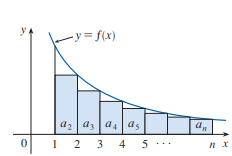
\includegraphics[width=0.35\textwidth]{graph74.png}
\end{figure}
\begin{figure}[htbp]
    \centering
    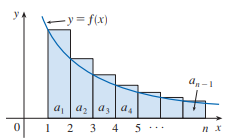
\includegraphics[width=0.35\textwidth]{graph75.png}
\end{figure}

\end{document}